\section{Vehicle-Aware Multi-Objective Optimization}
\label{sec:vehicle_aware}
Commercial logistics optimization requires balancing multiple conflicting operational goals.

\subsection{Multi-Objective Cost Formulation}
For a candidate solution $S$ represented by edge traversal variables $x_{ijk} \in \{0, 1\}$, the four objective metrics are:
\begin{align}
\mathcal{D}(\mathbf{x}) &= \sum_{k \in \mathcal{K}} \sum_{(i,j) \in \mathcal{E}} d_{ij} x_{ijk} \quad (\text{Total Distance}) \\
\mathcal{C}(\mathbf{x}) &= \sum_{k \in \mathcal{K}} \left( c_{\text{fixed}, k} y_k + \sum_{(i,j) \in \mathcal{E}} (c_{\text{dist}, k} d_{ij} + c_{\text{time}, k} t_{ij}) x_{ijk} \right) \\
\mathcal{E}(\mathbf{x}) &= \sum_{k \in \mathcal{K}} \sum_{(i,j) \in \mathcal{E}} (\mu_k f_k d_{ij}) x_{ijk} \quad (\text{Energy Consumption}) \\
\mathcal{M}(\mathbf{x}) &= \sum_{k \in \mathcal{K}} \sum_{(i,j) \in \mathcal{E}} (e_k \mu_k f_k d_{ij}) x_{ijk} \quad (\text{Carbon Emissions})
\end{align}

\subsection{Dimensionless Scalarization}
The scalarized fitness is evaluated against initial reference values $(\mathcal{D}_0, \mathcal{C}_0, \mathcal{E}_0, \mathcal{M}_0)$:
\begin{equation}
\min \quad \mathcal{F}(\mathbf{x}) = \alpha_1 \frac{\mathcal{D}(\mathbf{x})}{\mathcal{D}_0} + \alpha_2 \frac{\mathcal{C}(\mathbf{x})}{\mathcal{C}_0} + \alpha_3 \frac{\mathcal{E}(\mathbf{x})}{\mathcal{E}_0} + \alpha_4 \frac{\mathcal{M}(\mathbf{x})}{\mathcal{M}_0}
\end{equation}
subject to $\sum_{m=1}^4 \alpha_m = 1.0$.

Fig.~\ref{fig:soh_range} demonstrates the direct physical impact of battery degradation ($\text{SoH}$) and State of Charge ($\text{SoC}$) on usable operating range, reinforcing why nominal capacity assumptions lead to infeasible routing in practice.

\begin{figure}[t]
\centering
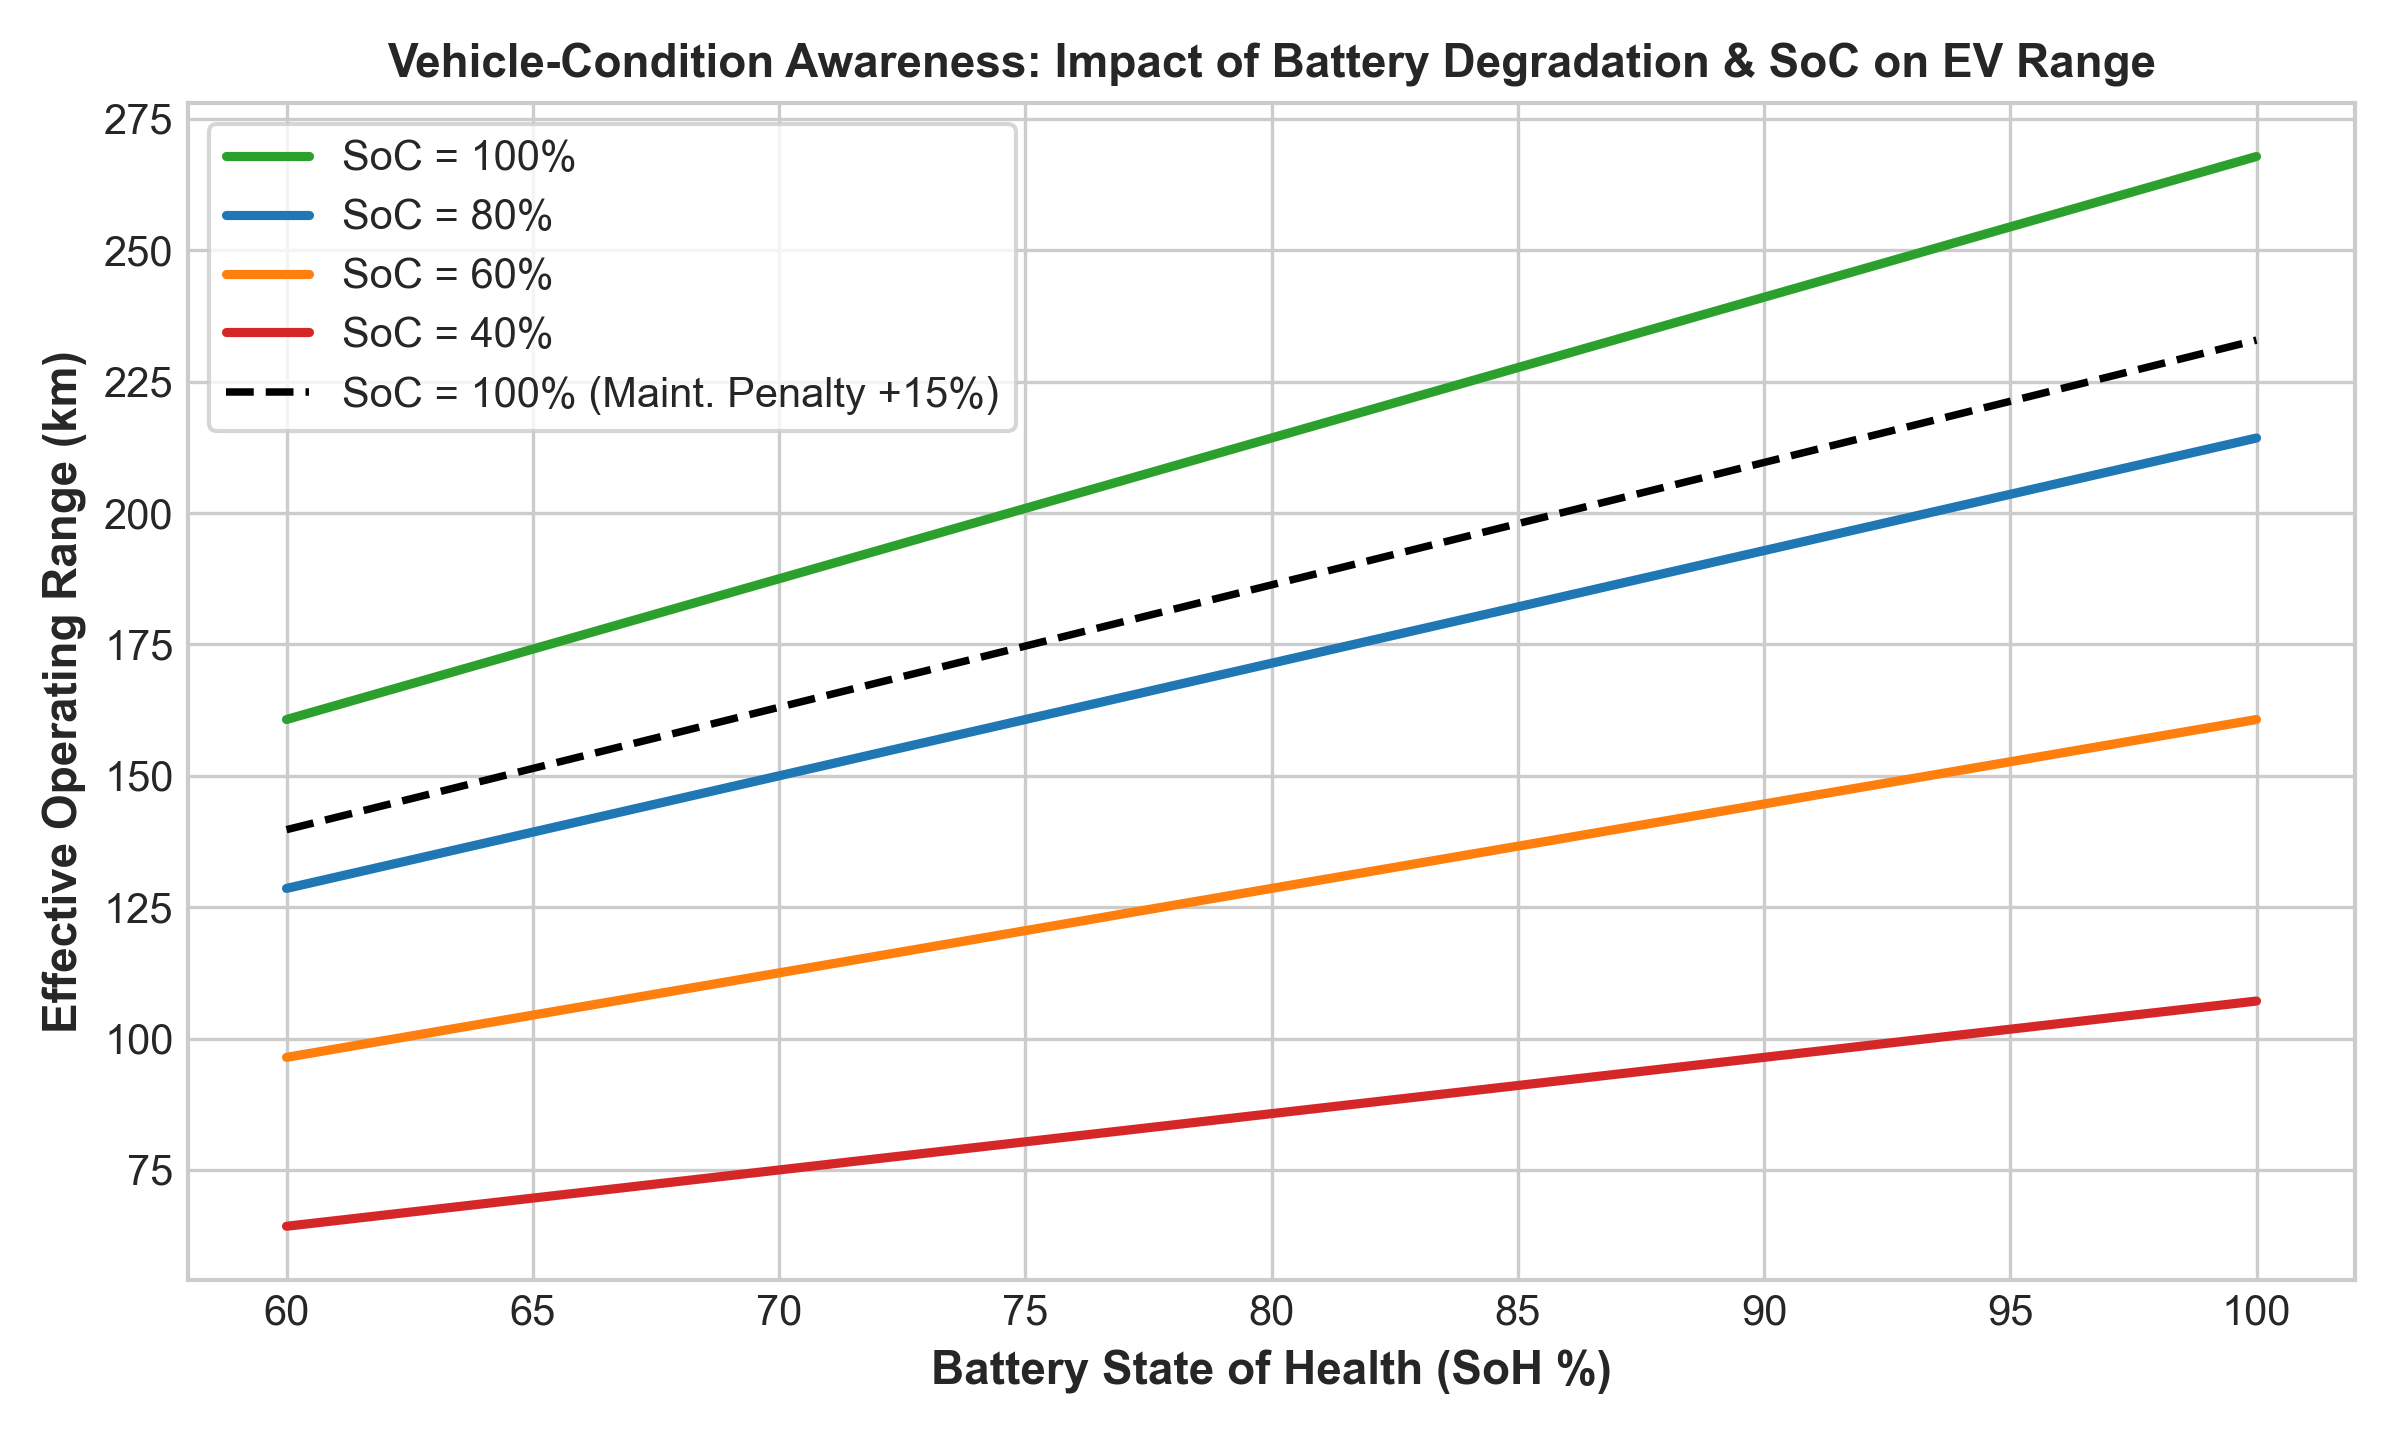
\includegraphics[width=0.48\textwidth]{figures/fig3_battery_soh_range.png}
\caption{Vehicle condition physics: impact of battery State of Health (SoH) and State of Charge (SoC) on usable EV range, with a 15\% maintenance wear penalty.}
\label{fig:soh_range}
\end{figure}
